\section{Define, in your own words, what a software product line is.}

\textbf{Definition in the slides}: A software product line (SPL) is about building a family of software systems sharing a common set of features that satisfy the needs of a particular domain. \\

\textbf{My definition}: Let’s take all the online banking applications, for example, Belfius, BNP Paribas, etc. They all allow the same kind of actions: logging in, seeing the amount of money you have, sending money to other persons, etc. We can generalize and say that they offer a \textbf{common set of features} and they represent a “\textbf{family of software}” which are “the online banking applications”. \\
The advantage and the goal of a \textbf{software product line}, here, is to allow the development of multiple online banking applications, one for each bank, by implementing only once the common set of features.\\

Developing applications in that way saves of course time and therefore money. It is called '\textbf{economies of scope}', which in other words means “savings from using technology to build a greater diversity of outputs with the same or less inputs”.

\section{Explain the difference between economies of scale and economies of scope, in the context
of software product lines.}

In factories, the \textbf{economies of scale} are possible because a lot of the same product has to be built. The factory is “super specialized” to build a specific product and is therefore very efficient.
In software engineering, the \textbf{economies of scope} are possible when the goal of the applications is somehow the same. In that case, a software product line can be created, which allows the developers to implement only once the common set of features and to re-use that set to create multiple applications. \\

The difference between both economies is simply that for the economies of scale, the \textbf{same product} is built a huge amount of times, while in the economies of scope, it’s a \textbf{family of software systems} that is built a lot of times. That means for the latter that the same application is (normally?) never built twice because each one of them is still a little specialized “for each client”.

\section{Explain what the main purpose of domain analysis is.
Explain and discuss the different phases of the domain analysis process.}

The main purpose of domain analysis is, for the developer, to \textbf{learn background information so that he understands the problem and can make good decisions about it}. The word ‘domain’ can mean a general domain such as ‘banking services’, ‘airline reservations’, etc or a more narrower domain such as ‘scheduling meetings’. Those who work in the domain and have a deep knowledge about it are called “\textbf{domain experts}”. Moreover, by having that knowledge of the domain, the developer can \textbf{discover the commonalities} among related software systems of that domain.\\

The domain analysis’ process is divided into three basic phases:
\begin{enumerate}
\item \textbf{Context analysis}: the domain analyst interacts with users and domain experts to \textbf{establish the bounds of the domain}. He gathers sources of information and \textbf{defines the scope of the analysis} by identifying the primary inputs and outputs of software in the domain.
\item \textbf{Domain modeling}: the domain analyst uses what he gathers from the context analysis to support the creation of a \textbf{domain model}. The domain model is reviewed by the user, domain expert, and requirements analyst. Such domain model can consist of several artifacts such as a feature model, a dictionary, an entity-relationship diagram, other diagrams, etc.
\item \textbf{Architecture modeling}: using the domain model, the domain analyst produces an \textbf{architecture model}. This model should be reviewed by the domain expert, the requirements analyst and the software engineer (not the user). This architecture model \textbf{captures the overall structure of the implementation} of different software systems in the domain.
\end{enumerate}

\section{What is feature-oriented domain analysis? What is a feature?
How does this relate to software product lines?}

\textbf{Feature-Oriented Domain Analysis} (FODA) is a particular domain analysis technique that focuses on the identification of prominent (=something you can’t miss) or distinctive features of software systems in a domain. With this technique, the developer can find the \textbf{commonalities} (what features are in common) and the \textbf{variabilities} (what features distinguish each software system).\\

A feature is a (prominent or distinctive) \textbf{user-visible aspect, quality or characteristic of the domain}. It describes a mandatory, optional or alternative characteristic of these related systems.\\

Domain analysis and more precisely Feature-Oriented Domain Analysis provides a \textbf{generic and reusable description of the requirements} of a class of systems. It defines what is common across all systems in that domain (which may lead to the creation of a software product line). That allows the developer to implement the common features as reusable components that may be reused across different systems.

\section{Explain and illustrate the feature modeling notation on a simple example.}

Feature modeling is used in domain analysis and software product lines to express the commonalities and variabilities of a family of systems in terms of features they may offer. It consists of a hierarchy of features.\\

\textbf{Mandatory features = must have}\\
\textbf{Optional features = may or may not have}\\
\textbf{Alternative features = one of the two, but can’t have both or none (XOR)}\\
\textbf{OR features = at least one}\\
\begin{center}
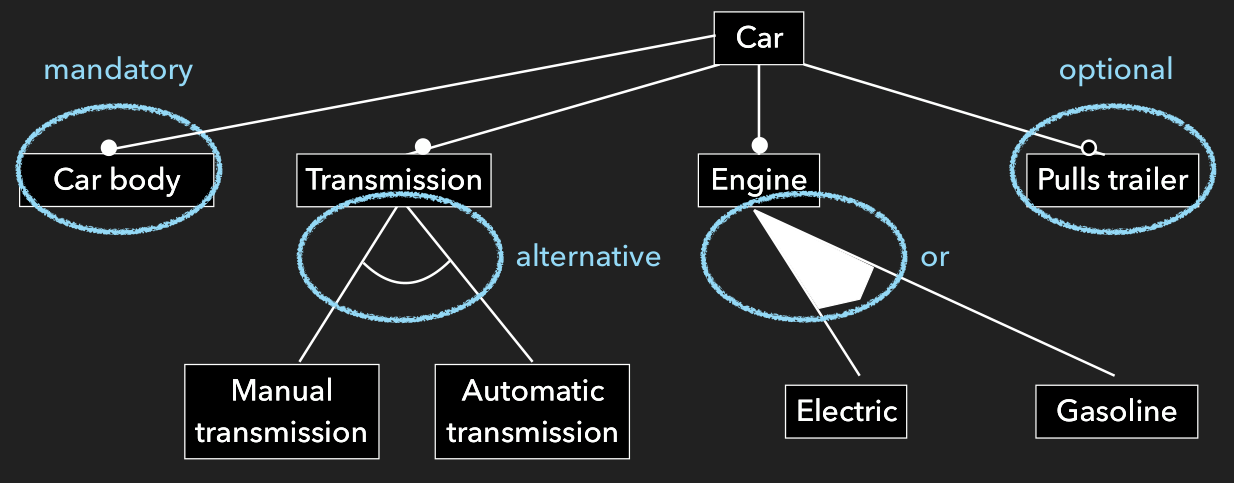
\includegraphics[scale=0.4]{FeatureModel.PNG}
\end{center}

\section{What is a configuration of a feature model? When is a configuration valid?
Explain and illustrate on an example. When is a feature model inconsistent?}

A configuration of a feature model can be pictured as one ‘instance’ of the feature model where some features have been chosen while others not. For example, with the above feature model of a car, a configuration represents a particular car.\\

A \textbf{valid configuration} is a configuration that \textbf{respects the semantics imposed by the dependencies and constraints} (= respects all the rules of the feature model). For example, a car can’t have a manual AND an automatic transmission at the same time.\\
\begin{center}
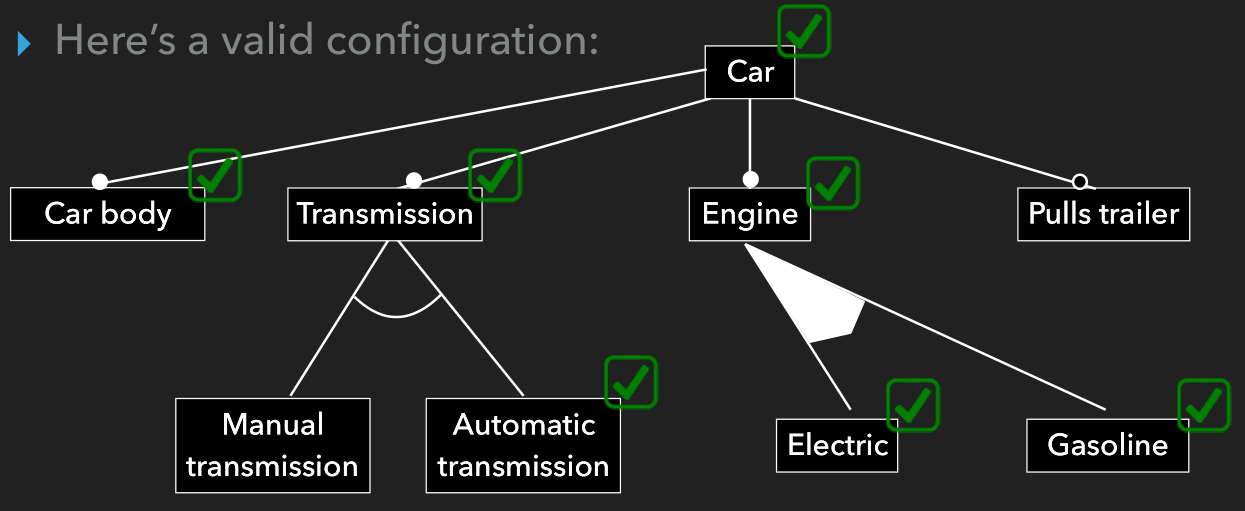
\includegraphics[scale=0.4]{FeatureModelValidConfiguration.PNG}
\end{center}
An \textbf{inconsistent feature model} is a feature model which does not have any valid configuration.


\section{Explain, in the context of feature modeling, the notions of commonality and variability.}

In the context of feature modeling, a \textbf{commonality} is a feature that appears in all of the feature model’s valid configuration. That feature can’t be taken out, it must be there. \\
On the other hand, a \textbf{variability} is a feature that appears only in some of the valid configurations. 
